% !TEX root = ../bachlor-arbeit.tex
To implement the desired algorithm we need to be able to calculate the optical behavior of stacked meta surfaces. The mathematical framework we will use is called Scatter Matrix Calculus and this section will give some insight into its physical origin and how to use it. We will start with the Maxwell Equations in matter.
\newlparagraph{Maxwell Equations}

\begin{tabular*}{\textwidth}{ll}
\begin{minipeqn}
    \curl{\vb{E}(\vb{r}, t)} = - \pdv{t} \vb{B}(\vb{r}, t)
\end{minipeqn}&
\begin{minipeqn}[c]
    \div \vb{D}(\vb{r}, t) = \rho_\s{ext}(\vb r, t)
\end{minipeqn}\\
\begin{minipeqn}
    \curl \vb H(\vb r, t) = \vb j(\vb r, t) + \pdv{t} \vb D(\vb r, t)
\end{minipeqn}&
\begin{minipeqn}[c]
    \div \vb B(\vb r, t) = 0
\end{minipeqn}
\end{tabular*}
\\
\\


The four involved fields are:
$\vb E$...electric field, $\vb B$...magnetic flux density, $\vb D$...electric flux density and $\vb H$...magnetic field and the sources are the external charges $\rho_\s{ext}$ and the macroscopic currents $j$. All the material properties are captured by the $\vb D$ and $\vb H$ fields which are defined as:


\begin{equation}\label{eq:bg:D}
\begin{aligned}
    \vb D(\vb r, t) &= \varepsilon_0 \vb E (\vb r, t) + \vb P (\vb r, t)\\
    \vb H(\vb r, t) &= \frac{1}{\mu_0} \qty[\vb B(\vb r, t) - \vb M(\vb r, t)]
\end{aligned}
\end{equation}


Where $\vb P$ is the dielectric polarization and $\vb M$ is the magnetic polarization. One can read equation \eqref{eq:bg:D} in the following way:
When the electric field $\vb E$ interacts with matter it exerts a force on all its charges and displaces them by a small amount. The separation of charges results in a counter field $\vb P$ and the total field $\vb D$ is now a superposition of $\vb E$ and $\vb P$.
This set of equations describes the whole electromagnetic spectrum, in this work however we are only interested in visible (VIS) and near infrared (NIR) light where we can make some simplifications. Generally in optics materials are non-magnetizable so $\vb M = 0$ and there are no free charges $\rho_\s{ext}$ = 0. Inserting these assumptions into the maxwell equation gives:
\\


\noindent
\begin{tabular*}{\textwidth}{ll}
\begin{minipeqn}\label{eq:bg:M1}
    \curl{\vb{E}(\vb{r}, t)} = - \mu_0 \pdv t \vb H(\vb r, t)
\end{minipeqn}&
\begin{minipeqn}[c]\label{eq:bg:M2}
    \varepsilon_0 \div \vb{E}(\vb{r}, t) = - \div \vb P(\vb r, t)
\end{minipeqn}\\
\begin{minipeqn}\label{eq:bg:M3}
    \curl \vb H(\vb r, t) = \vb j(\vb r, t) + \pdv{t} \vb P(\vb r, t)
    + \varepsilon_0 \pdv{t} \vb E(\vb r, t)
\end{minipeqn}&
\begin{minipeqn}[c]
    \div \vb H(\vb r, t) = 0
\end{minipeqn}
\end{tabular*}


\newlparagraph{Light in Vacuum}
Now we can derive the famous wave equation by considering $\curl$ \eqref{eq:bg:M1}:


\begin{equation}
\hspace{3cm}
\begin{aligned}
    \phantom{\Longleftrightarrow} \quad
    \curl \bigg [\curl \vb E \bigg ] &= \curl[- \mu_0 \pdv t \vb H]
    \\
    \Longleftrightarrow \quad
    \grad(\div \vb E) - \Delta \vb E &=
    - \mu_0 \pdv t \curl \vb H
    \qquad \bigg | \qq{subs. \eqref{eq:bg:M3} and \eqref{eq:bg:M2}}
    \\
    \Longleftrightarrow \quad \ \
    \frac{1}{c^2} \pdv[2] t \vb E - \Delta \vb E
    &= -\mu_0 \pdv t \vb j - \mu_0 \pdv[2] t \vb P +
    \frac{1}{\varepsilon_0} \grad(\div \vb P)
\end{aligned}
\end{equation}

In vacuum ($\vb P = 0$ and $\vb j = 0$) the right side of this equation vanishes and we are left with\\
$\frac{1}{c^2} \pdv[2] t \vb E - \Delta \vb E = 0$ which is solved by the plane wave $\vb E = \vb E_0 e^{i(\vb k \vb r - \omega t)}$ where $\frac{\omega}{k} = c$. This describes the propagation of light through empty space: a sinusoidal oscillation in time and space along the $\vb k$ direction where $\vb E, \, \vb B$ and $\vb k$ are all perpendicular to each other.
\note{this needs details} \note{show figure?}

\newlparagraph{Light in homogeneous, isotropic materials}\label{par:light_in_materials}
The next question we can answer is how light propagates through a homogeneous and isotropic material. For us, the dielectric polarization is some linear function of the electric field so $\vb P(\vb r, t) = \hat{\chi}(\omega, \vb r) \vb E(\vb r, t)$. An isotropic material behaves the same for all orientations of $\vb E$ that means $\hat{\chi}(\omega, \vb r)$ becomes a scalar function $\chi(\omega, \vb r)$. If the material is additionally homogeneous, that is the same everywhere independent of $\vb r$, then $\grad \chi(\omega, \vb r) = 0$. With equation \eqref{eq:bg:M2} this gives us $\div \vb P = 0$
and the wave equation simplifies to:

\begin{equation}
\begin{aligned}
    &\frac{\varepsilon}{c^2} \pdv[2] t \vb E - \Delta \vb E = 0\\
    \qq*{where} &\varepsilon \, \vb E := \qty(1 + \chi) \vb E = \vb E + \vb P
\end{aligned}
\end{equation}

That means light behaves in these materials exactly as it would in vacuum we only have to account for a decreased speed of light
$c' = \frac{c}{\sqrt{\varepsilon}} =: \frac{c}{n}$
with the refractive index $n$.
This is equivalent to a decreased wavelength
$\lambda' =: \frac{\lambda}{n}$
or an increased wave vector
$k' = \frac{2 \pi}{\lambda'} = n \, k$.
A complex valued $n := \eta + i \kappa$ even captures the possibility of an exponentially decaying field:

\begin{equation}
    \vb E = \vb E_0 e^{i(n \vb k \vb r - \omega t)}
    = \vb E_0 \
    \underbrace{e^{-\kappa \vb k \vb r}}_\s{
    decay} \
    \underbrace{e^{i(\eta \vb k \vb r - \omega t)}}_\s{
    oscillation}
\end{equation}

\newlparagraph{Interfaces}
The meta surface stacks we want to understand are obviously not one homogeneous material. Rather they contain many interfaces between different materials and we can again use the maxwell equations to predict how light will behave at such an interface.
\\

\begin{figure}[H]
    \centering
    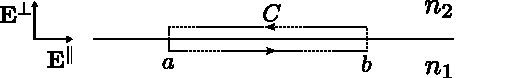
\includegraphics[width=.7\linewidth]{bg_interface}
    \caption{An interface of two materials with different refractive indices $n_1$ and $n_2$ and a closed contour $C$ which is tangent to the interface between the points $a$ and $b$.}
    \label{fig:bg:interface}
\end{figure}

Let us consider a closed contour $C$ around an interface as seen in Figure \ref{fig:bg:interface} and integrate the first maxwell equation \eqref{eq:bg:M1} over the surface $A$ enclosed by that contour:

\begin{equation}
\begin{aligned}
    \int_A \curl \vb E(\vb r, t) \, \dd \vb A
    &= - \mu_0 \pdv t \int_A \vb H(\vb r, t) \dd \vb A\\
    \overset{\s{stokes}}{\Longleftrightarrow} \hspace{3em}
    \int_{C = \partial A} \vb E(\vb r, t) \dd \vb r
    &= - \mu_0 \pdv t \int_A \vb H(\vb r, t) \dd \vb A\\
\end{aligned}
\end{equation}

But now we can bring the contour infinitely close to the interface and thus reduce the right hand side of the equation, the total magnetic flux, through the surface, to zero. That leaves us with:

\begin{equation}
\begin{aligned}
    \int_a^b \vb E_1 \, \dd \vb r \ &+ \int_b^a \vb E_2 \,  \dd \vb r = 0\\
    \Longleftrightarrow \hspace{3em}
    \int_a^b \vb E_1 \, \dd \vb r &= \int_a^b \vb E_2 \,  \dd \vb r \\
\end{aligned}
\end{equation}

Because $a$ and $b$ were chosen arbitrarily that means that the transverse field components along the path need to be continuous so
$\vb E_1^{\parallel} = \vb E_2^{\parallel}$.
The analog expression
$\vb H_1^{\parallel} = \vb H_2^{\parallel}$
can be shown by starting with the third maxwell equation \eqref{eq:bg:M3} instead. We can now use these continuity conditions to learn more about the behavior of light at these interfaces.

\begin{figure}[H]
    \centering
    \includegraphics[width=.7\linewidth]{bg_fresnel}
    \caption{Interface between two materials of different refractive indices $n_1$ and $n_2$. The incident light has a wave vector $\vb k^\s{i}$ and is partially transmitted and partially reflected. The fields are shown in transverse electric (TE) polarization where $\vb H$ is in the $x$-$z$ plane and $\vb E$ occilates in the $y$ direction.}
    \label{fig:bg:fresnel}
\end{figure}

Let us consider the same interface from before and have an incident field
$\vb E^\s{i}$ interact with it. From figure \ref{fig:bg:fresnel} we can see:

\begin{equation} \label{eq:bg:k}
    \vb k^\s{i} = k_0 n_1
    \begin{pmatrix}
        -\sin \varphi_\s{i}\\ 0\\ -\cos \varphi_\s{i}
    \end{pmatrix}
    , \
    \vb k^\s{r} = k_0 n_1
    \begin{pmatrix}
        \phantom{-} \sin \varphi_\s{r} \\ 0\\ -\cos \varphi_\s{r}
    \end{pmatrix}
    , \
    \vb k^\s{t} = k_0 n_2
    \begin{pmatrix}
        \sin \varphi_\s{t}\\ 0\\ \cos \varphi_\s{t}
    \end{pmatrix}
\end{equation}

Now we can decompose the electric field into two orthogonal polarizations. One component were $\vb E = E \, \va{e_y}$ called transverse electric (TE) as shown in figure \ref{fig:bg:fresnel} and its orthogonal component where $\vb H = H \, \va{e_y}$ called transverse magnetic (TM). If we apply the continuity condition from before to the TE component we get $\vb E_1 = \vb E_2$ at $z = 0$:

\begin{equation}
\begin{aligned}
    \vb E^\s{i} + \vb E^\s{r} &= \vb E^\s{t} \\
    E^\s{i} e^{i(k^\s{i}_x x)} + E^\s{r} e^{i(k^\s{r}_x x)}
    &= E^\s{t} e^{i(k^\s{t}_x x)}
\end{aligned}
\end{equation}

This is only possible for all $x$ if:

\begin{equation} \label{eq:bg:x}
    E^\s{i} + E^\s{r} = E^\s{t} \qq{and}
    k^\s{i}_x = k^\s{r}_x = k^\s{t}_x
\end{equation}

Two basic laws of optics lie in this relation: The law of reflection

\begin{equation}
    k^\s{i}_x = k^\s{r}_x
    \quad \Rightarrow \quad
    k_0 n_1 \sin \varphi_i =  k_0 n_1 \sin \varphi_r
    \quad \Rightarrow \quad
    \varphi_i = \varphi_r := \varphi_1
\end{equation}

and the Snells law of refraction

\begin{equation}
    k^\s{i}_x = k^\s{t}_x
    \quad \Rightarrow \quad
    k_0 n_1 \sin \varphi_i =  k_0 n_2 \sin \varphi_t
    \quad \Rightarrow \quad
    n_1 \sin \varphi_i = n_2 \sin \varphi_t
\end{equation}

\newlparagraph{Fresnel Equations}
To fully describe an interface we also need know the fraction of the transmitted
$t := E^t / E^i$
and the reflected
$r := E^r / E^i$ fields.
Again using the TE polarization we have an orientation of fields were $\vb E = E \, \va e_y$ and $\vb H$ is contained perpendicular to $\vb E$ in the $x$-$z$ plane:

\begin{equation} \label{eq:bg:H}
    \vb H^\s{i} = H^\s{i}
    \begin{pmatrix}
        -\cos \varphi_\s{i}\\ 0\\ -\sin \varphi_\s{i}
    \end{pmatrix}
    , \
    \vb H^\s{r} = H^\s{r}
    \begin{pmatrix}
        \cos \varphi_\s{r} \\ 0\\ \sin \varphi_\s{r}
    \end{pmatrix}
    , \
    \vb H^\s{t} = H^\s{t}
    \begin{pmatrix}
        -\cos \varphi_\s{t}\\ 0\\ \sin \varphi_\s{t}
    \end{pmatrix}
\end{equation}


The $H_x$ component is tangent to the interface so it also needs to be continuous across the boundary:

\begin{equation}\label{eq:bg:Hx}
\begin{aligned}
     H^\s{i}_x +  H^\s{r}_x &=  H^\s{t}_x \\
    \Longleftrightarrow \qquad
    H^\s i \cos \varphi_1 - H^\s r \cos \varphi_1 &= H^\s t \cos \varphi_2
    \qquad  \qquad
\end{aligned}
\end{equation}

Maxwells first equation \eqref{eq:bg:M1} allows us connect the magnitudes of $\vb H$ and $\vb E$ via the refractive index $H \sim n \, E$. This changes \eqref{eq:bg:Hx} to:

\begin{equation}
    n_1 \, E^\s i \cos \varphi_1 - n_1 \, E^\s r \cos \varphi_1 =
    n_2 \, E^\s t \cos \varphi_2
\end{equation}

Substituting $E^\s r$ or $E^\s i$ with \eqref{eq:bg:x} and rearranging we get:

\begin{equation}
    t = \frac{2 n_1 \cos \varphi_1}{n_1 \cos \varphi_1 + n_2 \cos \varphi_2}
    \qq{and}
    r = \frac{n_1 \cos \varphi_1 - n_2 \cos \varphi_2}{
    n_1 \cos \varphi_1 + n_2 \cos \varphi_2}
\end{equation}

These are called the Fresnel equations for the TE component. The TM component can be treated analogous which yields:

\begin{equation}
    t = \frac{2 n_1 \cos \varphi_1}{n_2 \cos \varphi_1 + n_1 \cos \varphi_2}
    \qq{and}
    r = \frac{n_2 \cos \varphi_1 - n_1 \cos \varphi_2}{
    n_2 \cos \varphi_1 + n_1 \cos \varphi_2}
\end{equation}

For perpendicular incident light at $\varphi = 90^\circ$ these should describe the same situation as we can no longer differentiate between TE and TM components and indeed for this angle they are equivalent if we consider that the TE factors describe the electric field and the TM factors describe the magnetic field. The TE factors become:

\begin{equation}
    t = \frac{2 n_1}{n_1 + n_2} \qq{and} r = \frac{n_1 - n_2}{n_1 + n_2}
\end{equation}

\newlparagraph{Stacking}
We can take this one step further by including interfaces which have incident light from both sides. Let $\vb E_\s{out}$ be the light coming out of the interface and $\vb E_\s{in}$ be the light going into the interface as seen in figure \ref{fig:bg:both}:

\begin{figure}[H]
    \centering
    \includegraphics[width=.6\linewidth]{bg_both_directions}
    \caption{Interface between two materials of different refractive indices $n_1$ and $n_2$ were incident light is coming from the front and the back.}
    \label{fig:bg:both}
\end{figure}

Using the factors from the Fresnel equations we get:

\begin{equation}
    E^b_\s{out} = E^f_\s{in} \, t^f + E^b_\s{in} \, r^b
    \qq{and}
    E^f_\s{out} = E^b_\s{in} \, t^b + E^f_\s{in} \, r^f
\end{equation}

This can concisely be expressed using matrices and vectors:

\begin{equation}
\begin{pmatrix}
    E^f_\s{out} \\
    E^b_\s{out}
\end{pmatrix} =
\underbrace{
\begin{pmatrix}
    t^f & r^b \\
    r^f & t^b
\end{pmatrix}
}_{
 =: \hat{S}
}
\begin{pmatrix}
    E^f_\s{in} \\
    E^b_\s{in}
\end{pmatrix}
\end{equation}

We call these matrices mapping field-in to field-out $S$-matrices. They can be used to describe more than just an interface. As shown in the paragraph \hyperref[par:light_in_materials]{Light in materials} when light propagates through homogeneous isotropic material just the phase changes by a factor of $e^{i k_0 n d}$ where $d$ is the distance traveled. We can express this by allowing complex valued $t$ and $r$:

\begin{equation}
    \hat S_{n, d} =
    \begin{pmatrix}
        e^{i k_0 n d} & 0 \\
        0 & e^{i k_0 n d}
    \end{pmatrix}
\end{equation}

Analogue the $S$-matrix for an interface from $n_1$ to $n_2$ is:

\begin{equation}
    \hat S_{n_1, n_2} =
    %increase matrix spacing for the fractions
    \begingroup
    \renewcommand*{\arraystretch}{1.5}
        \begin{pmatrix}
            \frac{2 n_1}{n_1 + n_2} & \frac{n_2 - n_1}{n_1 + n_2} \\
            \frac{n_1 - n_2}{n_1 + n_2} & \frac{2 n_1}{n_1 + n_2}
        \end{pmatrix}
    \endgroup
\end{equation}


Say we have a stack of different homogeneous isotropic materials. We are now are now able to write down an $S$-matrix for every part of the stack that is every interface and every propagation between interfaces as seen in figure \ref{fig:bg:star_prod}, but we cannot predict the behavior of the stack as a whole:

\begin{figure}[H]
    \centering
    \includegraphics[width=.6\linewidth]{bg_starprod}
    \caption{A slab of one homogeneous isotropic material with thickness $d$ in air $(n_0)$. This setup is described by two interface and one propergation $S$-matrices.}
    \label{fig:bg:star_prod}
\end{figure}



The combined $S$-matrix $\hat S$ consisting of $\hat S_1$ and $\hat S_2$ cannot be obtained by simply using the matrix product. The result would be:

\begin{equation}
    \hat S_1 \, \hat S_2 =
    \begin{pmatrix}
        t^f_1 \, t^f_2 + r^b_1 \, r^f_2 & t^f_1 \, r^b_2 + r^b_1 \, t^b_2 \\
        r^f_1 \, t^f_2 + t^b_1 \, r^f_2 & r^f_1 \, r^b_2 + t^b_1 \, t^b_2
    \end{pmatrix} \neq
    \begin{pmatrix}
        t^f & r^b \\
        r^f & t^b
    \end{pmatrix} =
    \hat S
\end{equation}

and this would imply that the transmission from the front $t^f$ increases when the internal reflections of the system $r^b_1$ and $r^f_2$ increase which is the opposite of the behavior we expect. Redheffer \cite{Redheffer1960} studied these kind of systems in the 60s and found an operator $\star$ which yields the combined $S$-matrix:

\begin{equation}\label{eq:bg:star}
    \hat S_1 \star \hat S_2 :=
    \begin{pmatrix}
        t^f_2 (1 - r^b_1 r^f_2)^{-1} t^f_1 &
        r^b_2 + t^f_2 r^b_1 (1 - r^f_2 r^b_1)^{-1} t^b_2\\
        r^f_1 + t^b_1 r^f_2 (1 - r^b_1 r^f_2)^{-1} t^f_1 &
        t^b_1 (1 - r^f_2 r^b_1)^{-1} t^b_2
    \end{pmatrix}
\end{equation}

For this operation to produce physically valid results certain condition have to be met. We will discuss these in detail in the paragraph \hyperref[par:conditions]{Conditions} of section \ref{sec:SASA}.
Applied to the example of figure \ref{fig:bg:star_prod} that gives:

\begin{equation}
    \hat S = \hat S_{n, n_0} \star \hat S_{n, d} \star \hat S_{n_0, n}
\end{equation}

Notice the order in which the matrices appear in the product where the physically first matrix appears last in the product. More on that also in section \ref{sec:SASA}.


\newlparagraph{Polarization}
Up to this point we are dealing with vectors of the form
$
\begin{pmatrix}
    E^f_\s{in} \\
    E^b_\s{in}
\end{pmatrix}
$
where $E^f_\s{in}$ and $E^b_\s{in}$ are scalar properties. That means we can only describe linear polarized light in one direction. The last generalization we want to make is to extend this formalism to all polarizations. As shown in the paragraph \hyperref[par:light_in_materials]{Light in materials} a planar light wave propagating along the $z$ axis through a homogeneous isotropic material can be described as:

\begin{equation}
   \vb E =
   \begin{pmatrix}
       E_x e^{i(kz - \omega t + \varphi_x)}\\
       E_y e^{i(kz - \omega t + \varphi_y)}\\
       0\\
   \end{pmatrix}
   =
   \qty(E_x \, e^{i \varphi_x} \, \va{e_x} +
        E_y \, e^{i \varphi_y} \, \va{e_y})
       e^{i(kz - \omega t)}
\end{equation}
\\

\noindent
the waves polarization is determined by the scaling factors of $\va{e_x}$ and $\va{e_y}$ and can be expressed as a \textit{Jones Vector} $\vb j \in \mathbb{C}^2$.

\begin{equation}
   \vb j = \frac{1}{\sqrt{E_x^2 + E_y^2}}
   \begin{pmatrix}
       E_x\\
       E_y \, e^{i \delta}
   \end{pmatrix}
   \qq{with}
   \delta := \varphi_y - \varphi_x
\end{equation}

\noindent
Now all linear operations on the polarization are matrices $\hat{M} \in \mathbb{C}^{2 \times 2}$. That means all passive components have a corresponding matrix. A couple examples for components in horizontal position:


\begin{equation}
\begin{split}
   \qq*{polarizer:} \hat{M} &=
   \begin{pmatrix}
       1 & 0\\
       0 & 0
   \end{pmatrix}\\
   \qq*{$\lambda / 4$ plate:} \hat{M} &=
   \begin{pmatrix}
       1 & 0\\
       0 & i
   \end{pmatrix}
   e^{-\frac{i \pi}{4}}\\
   \qq*{$\lambda / 2$ plate:} \hat{M} &=
   \begin{pmatrix}
       -i & 0\\
       0 & i
   \end{pmatrix}\\
\end{split}
\end{equation}

We can now generalize the $S$-matrix Calculus simply by allowing proper Jones matrices in place of the Fresnel factors: $t \rightarrow \hat T$ and $r \rightarrow \hat R$. The star product of two $S$-matrices becomes:

\begin{equation}\label{eq:bg:star}
    \hat S_1 \star \hat S_2 =
    \begin{pmatrix}
        \hat T^f_1 & \hat R^b_1 \\
        \hat R^f_1 & \hat T^b_1
    \end{pmatrix}
    \star
    \begin{pmatrix}
        \hat T^f_2 & \hat R^b_2 \\
        \hat R^f_2 & \hat T^b_2
    \end{pmatrix}
    =
    \begin{pmatrix}
        \hat T^f_2 (\mathbb 1 - \hat R^b_1 \hat R^f_2)^{-1} \hat T^f_1 &
        \hat R^b_2 + \hat T^f_2 \hat R^b_1 (\mathbb 1 - \hat R^f_2 \hat R^b_1)^{-1} \hat T^b_2\\
        \hat R^f_1 + \hat T^b_1 \hat R^f_2 (\mathbb 1 - \hat R^b_1 \hat R^f_2)^{-1} \hat T^f_1 &
        \hat T^b_1 (\mathbb 1 - \hat R^f_2 \hat R^b_1)^{-1} \hat T^b_2
    \end{pmatrix}
\end{equation}

So the general $S$-matrix is $\hat S \in \mathbb C^{4 \times 4}$ and consist of four separate Jones matrices.
